\documentclass[11pt]{article}
\usepackage[margin=1.5cm]{geometry}
\usepackage{amsmath}
\usepackage{tikz}
\usetikzlibrary{arrows.meta, positioning, shapes.geometric, calc, fit, graphs,
                decorations.pathmorphing, decorations.pathreplacing,
                decorations.shapes, decorations.markings, automata, shadows, math}
\usetikzlibrary{
    arrows.meta,
    fit,
    automata,
    positioning,
    shadows,
    calc,
    math,
    shapes.geometric,
    decorations,
    decorations.pathmorphing,
    decorations.pathreplacing,
    decorations.shapes,
    decorations.markings,
    graphs
}

\tikzset{%
   % Copy tensor node: a true circle shape, so edges anchor exactly on
   % the drawn circle instead of stopping at a text glyph's bounding box.
   copydot/.style={
      circle,
      draw,
      inner sep=0pt,
      outer sep=0pt,
      minimum size=3pt
   },
   dot/.style={
      circle,
      inner sep=0mm,
      outer sep=0mm,
      minimum size=2mm,
      draw=black,
      fill=black
   },
    triple/.style={
      double distance=2pt,
      postaction={draw}
    },
    quadruple/.style={
      double,
      double distance=2pt,
      postaction={
        draw,
        transform canvas={yshift=-.4pt},
      },
      postaction={
        draw,
        transform canvas={yshift=.4pt},
      }
    },
   every loop/.style={},
   d/.style={
     Circle[]-,
     shorten <=-2pt,
     transform canvas={shift={(-3pt, 4pt)}}
   },
   d0/.style={
     Circle[]-,
     shorten <=-2pt,
   },
   d1/.style={
     Circle[]-,
   },
   dn/.style={
     draw, circle, minimum size=1.3em
   },
   ddn/.style={
     draw, circle, double, minimum size=1.3em
   },
   dddn/.style={
     draw, circle, double, minimum size=1.3em,
       double distance=2pt,
       postaction={draw}
   },
   triangle/.style={
    regular polygon,
    regular polygon sides=3,
    rotate=270,
    scale=.5,
    inner sep=3pt,
    draw
   },
   % A double wire with a half-twist: the two wires cross once, so the
   % top/bottom reading order is preserved through a 180-degree turn.
   twist/.style={
      double,
      postaction={decorate, decoration={markings,
         mark=at position 0.5 with {
            \fill[white] (-.1,-.03) rectangle (.1,.03);
            \draw (-.1,.0176) .. controls (-.025,.0176) and (.025,-.0176) .. (.1,-.0176);
            \draw[white, line width=1.2pt] (-.1,-.0176) .. controls (-.025,-.0176) and (.025,.0176) .. (.1,.0176);
            \draw (-.1,-.0176) .. controls (-.025,-.0176) and (.025,.0176) .. (.1,.0176);
         }}}
   },
}



\newcount\traceitemcount

\newcommand{\trace}[2]{% #1 is the list of items, #2 is the looseness for the loop
   %\pgfmathsetmacro{\negspace}{-1.0em - 0.5em*#2} % Calculate negative space
   \hspace{-1em}
    \begin{tikzpicture}[baseline=(node1.base), inner sep=1pt]
        % Initialize a counter for tracking the number of items
        \traceitemcount=0
        
        % Define nodes
        \def\lastnode{node1}
        \foreach \i [count=\c] in {#1} {
            \ifnum \c=1
                \node (node\c) {$\i$}; % First node
            \else
                \node[right=1em of \lastnode] (node\c) {$\i$}; % Subsequent nodes
                \draw (\lastnode) -- (node\c); % Draw edge from last node to current
            \fi
            \global\advance\traceitemcount by 1
            \xdef\lastnode{node\c}
        }
        
        % Draw the loop edge
        \ifnum \traceitemcount=1
            \path (node1) edge [out=160, in=20, loop] ();
        \else
            \path (node1) edge [out=160, in=20, looseness=#2] (\lastnode);
        \fi
    \end{tikzpicture}
   \hspace{-1em}
}

\def\matmul#1{
   \vecmatvec{.5em}{}{#1}{}
}

\def\vecmatvec#1#2#3#4{
   \begin{tikzpicture}[baseline=-.25em, inner sep=1pt]
      \node (node0) {$#2$};
      \xdef\lastnode{node0}
      \foreach \i [count=\c] in {#3} {
         \node[right=#1 of \lastnode] (node\c) {$\i$};
         \draw (\lastnode.east) -- (node\c);
         \xdef\lastnode{node\c}
      }
      \node[right=#1 of \lastnode] (last) {$#4$};
      \draw (\lastnode.east) -- (last);
   \end{tikzpicture}
}

\def\detstack#1{
   \mathbin{\begin{tikzpicture}[baseline=(a0.base), inner sep=1pt]
      \node (a0) {#1};
      \node[right=.5em of a0] (dots) {$\cdots$};
      \node[right=.5em of dots] (a1) {#1};
      \draw (a0.north) -- ++(0,.2) coordinate (a0top);
      \draw (a1.north) -- ++(0,.2) coordinate (a1top);
      \draw (a0.south) -- ++(0,-.2) coordinate (a0bot);
      \draw (a1.south) -- ++(0,-.2) coordinate (a1bot);
      \draw[line width=2pt] (a0top -| a0.west) -- (a1top -| a1.east);
      \draw[line width=2pt] (a0bot -| a0.west) -- (a1bot -| a1.east);
   \end{tikzpicture}}
}

% Penrose derivative loop: \dloop[<dot angle>]{<fit spec>} draws an ellipse
% around the given nodes with a filled dot ON the loop at the given angle.
% Names the ellipse node `dE` and the dot coordinate (ddot); whiskers are
% drawn afterwards from (ddot). Following Penrose, the row whisker bends
% left and the column whisker bends right (see \dwhiskers / \dwhiskersdown).
\newcommand{\dloop}[2][55]{%
   \node[ellipse, draw, inner sep=2.5pt, fit=#2] (dE) {};%
   \fill (dE.#1) circle (1.4pt);%
   \coordinate (ddot) at (dE.#1);%
}
\newcommand{\dwhiskers}{%
   \draw (ddot) .. controls +(80:.12) .. ++(-.2,.28);%
   \draw (ddot) .. controls +(45:.12) .. ++(.28,.18);%
}
\newcommand{\dwhiskersdown}{%
   \draw (ddot) .. controls +(280:.12) .. ++(-.2,-.28);%
   \draw (ddot) .. controls +(315:.12) .. ++(.28,-.18);%
}

% Define a new command for drawing the ellipse
\NewDocumentCommand{\drawellipse}{m m m m m o}{
    \def\centerX{#1}
    \def\centerY{#2}
    \def\widthR{#3}
    \def\heightR{#4}
    \def\angle{#5}
    
    \draw (\centerX,\centerY) ellipse [x radius=\widthR, y radius=\heightR];
    \fill ({\centerX + \widthR*cos(\angle)},{\centerY + \heightR*sin(\angle)}) circle [radius=0.075];
    
    % If target node is provided, use it, otherwise fall back to default behavior
    \IfNoValueTF{#6}{
        \draw ({\centerX + \widthR*cos(\angle)},{\centerY + \heightR*sin(\angle)}) -- ({\centerX + .5 + \widthR*cos(\angle)}, {\centerY + \heightR*sin(\angle)});
    }{
        \draw ({\centerX + \widthR*cos(\angle)},{\centerY + \heightR*sin(\angle)}) -- (#6);
    }
}

\usepackage[most]{tcolorbox}
\tcbset{listing side text, size=small, fonttitle=\bfseries,
        colback=black!2, colframe=black!40, listing options={
        basicstyle=\ttfamily\scriptsize, breaklines=true}}

% ---- approach A: legs key (candidate library code) ----
\makeatletter
\tikzset{
  tn/.style={inner sep=1pt, baseline=-.25em},
  every leg/.style={},
  every leg label/.style={font=\tiny},
  leg length/.initial=.35,
  legs/.style={append after command={\pgfextra{\def\tn@legopt{}\tn@legs{#1}}}},
  double legs/.style={append after command={\pgfextra{\def\tn@legopt{double}\tn@legs{#1}}}},
}
\def\tn@legs#1{\foreach \tn@item in {#1}{\expandafter\tn@leg\tn@item//\@nil}}
\def\tn@leg#1/#2/#3\@nil{%
  % Border point along the PAGE-coordinate direction #1 (handles rotated
  % shapes, unlike numeric anchors) so wide nodes don't eat the leg.
  \pgfpointshapeborder{\tikzlastnode}{\pgfpointadd{%
     \pgfpointanchor{\tikzlastnode}{center}}{\pgfpointpolar{#1}{10pt}}}%
  \pgfgetlastxy{\tn@bx}{\tn@by}%
  \if\relax\detokenize{#2}\relax
    \expandafter\draw\expandafter[\tn@legopt, every leg] (\tn@bx,\tn@by) -- ++(#1:\pgfkeysvalueof{/tikz/leg length});%
  \else
    \pgfmathsetmacro\tn@anch{#1+180}%
    \expandafter\draw\expandafter[\tn@legopt, every leg] (\tn@bx,\tn@by) -- ++(#1:\pgfkeysvalueof{/tikz/leg length})
       node[every leg label, anchor=\tn@anch, inner sep=1.5pt] {$#2$};%
  \fi}
\makeatother
% ---- approach D: kron pic (for the bundle comparison) ----
\tikzset{
  pics/kron/.style 2 args={code={
    \node[triangle, rotate=180] (-in) at (0,0) {};
    \node (-A) at (.6,.25) {#1};
    \node (-B) at (.6,-.25) {#2};
    \node[triangle] (-out) at (1.2,0) {};
    \draw (-in) -- (-A) -- (-out);
    \draw (-in) -- (-B) -- (-out);
  }},
}

\pagestyle{empty}
\setlength\parindent{0pt}
\begin{document}

\section*{Stress test: approach A on the book's hard diagram families}
Old code is verbatim from the chapters. Line counts include
\texttt{begin}/\texttt{end}.

% =====================================================================
\subsection*{S1. Eigendecomposition (1.1) --- copy dot with hanging $\lambda$}

\begin{tcblisting}{title={OLD (11 lines)}}
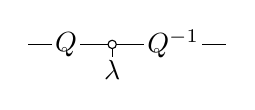
\begin{tikzpicture}[baseline=(Q.base), inner sep=1pt]
\node (Q) {$Q$};
\draw (Q.west) -- ++(-.3, 0);
\node[right=1em of Q, copydot] (dot) {};
\path (Q) edge (dot);
\node[below=.3em of dot] (e) {$\lambda$};
\path (dot) edge (e);
\node[right=1em of dot] (Qi) {$Q^{-1}$};
\path (dot) edge (Qi);
\draw (Qi.east) -- ++(.3, 0);
\end{tikzpicture}
\end{tcblisting}

\begin{tcblisting}{title={NEW (7 lines)}}
\begin{tikzpicture}[tn, baseline=(Q.base),
    every leg label/.style={}]
  \node[legs={180}] (Q) {$Q$};
  \node[right=1em of Q, copydot,
        legs={270/\lambda}] (dot) {};
  \node[right=1em of dot, legs={0}] (Qi) {$Q^{-1}$};
  \draw (Q) -- (dot) -- (Qi);
\end{tikzpicture}
\end{tcblisting}

% =====================================================================
\subsection*{S2. Strassen star (decompositions) --- hyperedge + 6 dangling legs}

\begin{tcblisting}{title={OLD (19 lines)}}
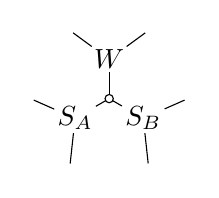
\begin{tikzpicture}[inner sep=1pt, baseline=.0em]
    \node[copydot] (m) at (0,0) {};
    \node (W) at (0,.5) {$W$};
    \node (SB) at (-30:.5) {$S_B$};
    \node (SA) at (-150:.5) {$S_A$};
    \node (w1) at (60:1) {};
    \node (w2) at (120:1) {};
    \node (sa1) at (-120:1) {};
    \node (sa2) at (-180:1) {};
    \node (sb1) at (-0:1) {};
    \node (sb2) at (-60:1) {};
    \draw (m) -- (W);
    \draw (m) -- (SA);
    \draw (m) -- (SB);
    \draw (W) -- (w1) {};
    \draw (W) -- (w2) {};
    \draw (SB) -- (sb1) {};
    \draw (SB) -- (sb2) {};
    \draw (SA) -- (sa1) {};
    \draw (SA) -- (sa2) {};
\end{tikzpicture}
\end{tcblisting}

\begin{tcblisting}{title={NEW (8 lines)}}
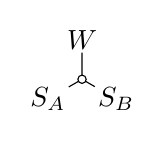
\begin{tikzpicture}[tn, baseline=0em, leg length=.5]
  \node[copydot] (m) at (0,0) {};
  \node[legs={60,120}]    (W)  at (0,.5)    {$W$};
  \node[legs={-120,180}]  (SA) at (-150:.5) {$S_A$};
  \node[legs={0,-60}]     (SB) at (-30:.5)  {$S_B$};
  \draw (m) -- (W)  (m) -- (SA)  (m) -- (SB);
\end{tikzpicture}
\end{tcblisting}

% =====================================================================
\subsection*{S3. Kronecker sandwich (511) LHS --- where A does NOT win}

\begin{tcblisting}{title={OLD (16 lines)}}
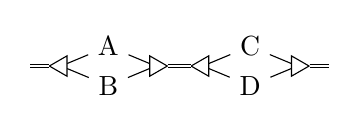
\begin{tikzpicture}[baseline=-.25em]
   \node[triangle, rotate=180] (F0) at (0,0) {};
   \node (A) at (.6,.25) {A};
   \node (B) at (.6,-.25) {B};
   \node[triangle] (F1) at (1.2,0) {};
   \draw[double] (F0) -- ++(-.4,0);
   \draw (F0) -- (A) -- (F1);
   \draw (F0) -- (B) -- (F1);
   \node[triangle, rotate=180] (F2) at (1.8,0) {};
   \node (C) at (2.4,.25) {C};
   \node (D) at (2.4,-.25) {D};
   \node[triangle] (F3) at (3,0) {};
   \draw (F2) -- (C) -- (F3);
   \draw (F2) -- (D) -- (F3);
   \draw[double] (F1) -- (F2);
   \draw[double] (F3) -- ++(.4,0);
\end{tikzpicture}
\end{tcblisting}

Approach A alone: essentially the same 16 lines (legs only replace the two
outer double stubs --- the triangles and fan wiring remain hand-placed).
The saving comes from approach D's molecule:

\begin{tcblisting}{title={NEW via D (7 lines)}}
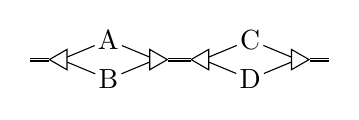
\begin{tikzpicture}[tn]
  \pic (k1) {kron={A}{B}};
  \pic (k2) at (1.8,0) {kron={C}{D}};
  \draw[double] (k1-in) -- ++(-.4,0);
  \draw[double] (k1-out) -- (k2-in);
  \draw[double] (k2-out) -- ++(.4,0);
\end{tikzpicture}
\end{tcblisting}

% =====================================================================
\subsection*{S4. (511b) --- bent identity wires: honest tie}

\begin{tcblisting}{title={OLD (17 lines) --- A offers nothing here}}
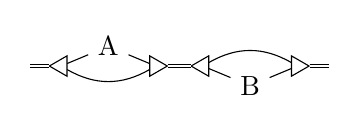
\begin{tikzpicture}[baseline=-.25em]
   \node[triangle, rotate=180] (F0) at (0,0) {};
   \draw[double] (F0) -- ++(-.4,0);
   \node (A) at (.6,.25) {A};
   \node[triangle] (F1) at (1.2,0) {};
   \draw (F0) -- (A) -- (F1);
   \draw (F0) edge[bend right] (F1);
   \node[triangle, rotate=180] (F2) at (1.8,0) {};
   \node (D) at (2.4,-.25) {B};
   \node[triangle] (F3) at (3,0) {};
   \draw (F2) edge[bend left] (F3);
   \draw (F2) -- (D) -- (F3);
   \draw[double] (F1) -- (F2);
   \draw[double] (F3) -- ++(.4,0);
\end{tikzpicture}
\end{tcblisting}

Bends between named nodes are already minimal in plain TikZ; a library can
only add a \texttt{kron} pic variant with an identity wire. Verdict: tie.

% =====================================================================
\subsection*{S5. Moment tensor $M_4$ --- existing macros already win}

\begin{tcblisting}{title={OLD (8 lines, uses \char`\\vecmatvec)}}
$M_4 =
\renewcommand*{\arraystretch}{1.3}
\begin{bmatrix}
   \vecmatvec{1em}{\tilde x}{}{} \\
   \vecmatvec{1em}{\tilde x}{}{} \\
   \vecmatvec{1em}{\tilde x}{}{} \\
   \vecmatvec{1em}{\tilde x}{}{}
\end{bmatrix}$
\end{tcblisting}

The book's \texttt{\char`\\vecmatvec}, \texttt{\char`\\trace},
\texttt{\char`\\detstack} macros are already the right abstraction for their
patterns. Approach A complements them; it should not replace them.

% =====================================================================
\subsection*{S6. Order-4 tensor with labeled legs --- A's best case}

\begin{tcblisting}{title={OLD style (9 lines)}}
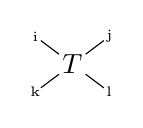
\begin{tikzpicture}[baseline=-.25em, inner sep=1pt]
   \node (T) {$T$};
   \draw (T) -- ++(-.4,.3)
      node[pos=1.3, font=\tiny] {i};
   \draw (T) -- ++(.4,.3)
      node[pos=1.3, font=\tiny] {j};
   \draw (T) -- ++(-.4,-.3)
      node[pos=1.3, font=\tiny] {k};
   \draw (T) -- ++(.4,-.3)
      node[pos=1.3, font=\tiny] {l};
\end{tikzpicture}
\end{tcblisting}

\begin{tcblisting}{title={NEW (3 lines)}}
\begin{tikzpicture}[tn]
  \node[legs={143/i, 37/j, 217/k, -37/l}] (T) {$T$};
\end{tikzpicture}
\end{tcblisting}

% =====================================================================
\subsection*{S7. Delete-the-node figure --- both sides, verbatim}

\begin{tcblisting}{title={OLD (10 + 9 lines, verbatim)}}
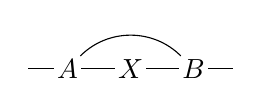
\begin{tikzpicture}[baseline=-.25em, inner sep=1pt]
   \node (A) at (0,0) {$A$};
   \node (X) at (.8,0) {$X$};
   \node (B) at (1.6,0) {$B$};
   \draw (A) -- (X);
   \draw (X) -- (B);
   \draw (A) edge[bend left=45] (B);
   \draw (A) -- ++(-.5,0);
   \draw (B) -- ++(.5,0);
\end{tikzpicture}
$=$
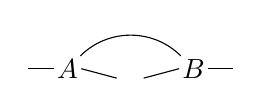
\begin{tikzpicture}[baseline=-.25em, inner sep=1pt]
   \node (A) at (0,0) {$A$};
   \node (B) at (1.6,0) {$B$};
   \draw (A) edge[bend left=45] (B);
   \draw (A) -- ++(-.5,0);
   \draw (B) -- ++(.5,0);
   \draw (A.east) -- ++(.45,-.12);
   \draw (B.west) -- ++(-.45,-.12);
\end{tikzpicture}
\end{tcblisting}

\begin{tcblisting}{title={NEW (7 + 6 lines)}}
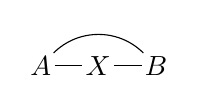
\begin{tikzpicture}[tn]
  \node[legs={180}] (A) {$A$};
  \node[right=1em of A] (X) {$X$};
  \node[right=1em of X, legs={0}] (B) {$B$};
  \draw (A) -- (X) -- (B);
  \draw (A) edge[bend left=45] (B);
\end{tikzpicture}
$=$
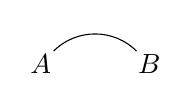
\begin{tikzpicture}[tn]
  \node[legs={180, -20}] (A) {$A$};
  \node[right=2.9em of A, legs={0, 200}] (B) {$B$};
  \draw (A) edge[bend left=45] (B);
\end{tikzpicture}
\end{tcblisting}

Modest win: the deleted-node stubs are just more legs
(\texttt{legs=\{180, -20\}}).

% =====================================================================
\subsection*{Verdict}

\begin{tabular}{llll}
Family & Old & New & Winner \\\hline
Derivative rows (loops) & 8--12 & 5--7 & A + \texttt{\char`\\dloop} \\
Labeled-leg tensors, TT chains & 6--10 & 2--4 & A (big) \\
Stars / hyperedges (Strassen) & 19 & 8 & A (big) \\
Copy-dot chains (eigen, Hadamard) & 11 & 7 & A (modest) \\
Bundle sandwiches (Kronecker) & 14--17 & 6--7 & D pics, not A \\
Bent wires, twists, wraps & --- & --- & tie: plain TikZ \\
\texttt{\char`\\vecmatvec}/\texttt{\char`\\trace}/\texttt{\char`\\detstack} rows & 1--8 & --- & existing macros \\
\end{tabular}

\medskip
A is the right \emph{foundation} (it never loses, wins wherever legs and
labels dominate), D's pics handle the recurring molecules, and the existing
macros stay. The one honest gap: nothing shortens bent-wire plumbing.

\end{document}
